\chapter{Images as Functions}

An Image as a function $ f $ from $ \mathbb{R}^2 $ to $ \mathbb{R}^M $:
\begin{itemize}
    \item $ f(x,y) $ gives the intensity at position $ (x,y) $
    \item Defined over a rectangle with a finite range:
    $ f: [a,b] \times [c,d] \rightarrow [0,255] $
    \item Pixel values:
    \begin{itemize}
        \item \textbf{Grayscale/Intensity}: $[0,255]$
        \item \textbf{Color (RGB)}: $[R, G, B]$
    \end{itemize}
\end{itemize}

\paragraph{Note:} Images are usually digital (\textbf{discrete}).

\subsection{Image Gradient}
\begin{itemize}
    \item Image gradient:
    $$
    \nabla f = \left[\frac{\partial f}{\partial x}, \frac{\partial f}{\partial y}\right]
    $$
    \item Gradient magnitude:
    $$
    \|\nabla f\| = \sqrt{\left(\frac{\partial f}{\partial x}\right)^2 + \left(\frac{\partial f}{\partial y}\right)^2}
    $$
    \item Gradient direction: Points in the direction of most rapid intensity change.
\end{itemize}

% --- Placeholder for image "VisualizingImageGradient.png" ---
\begin{figure}[htbp]
    \centering
    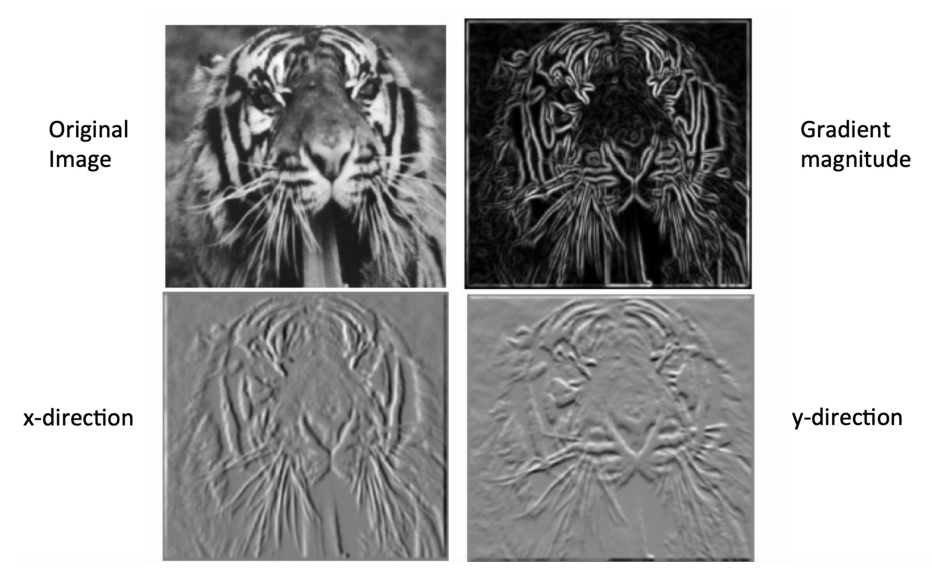
\includegraphics[scale=0.3]{figures/VisualizingImageGradient.png}
    \caption{Visualization of image gradient.}
\end{figure}

\clearpage

\subsection{Filters}
\begin{itemize}
    \item \textbf{Filtering}: Process to generate a new image by combining original pixel values.
    $$
    f[n] \rightarrow \text{System } \mathcal{G} \rightarrow h[n], \quad h = \mathcal{G}(f), \quad h[n] = \mathcal{G}(f)[n]
    $$
    \item \textbf{Linear filtering}: A system $ \mathcal{G} $ is linear if:
    $$
    \mathcal{G}(\alpha f + \beta g) = \alpha \mathcal{G}(f) + \beta \mathcal{G}(g)
    $$
    \item \textbf{Discrete convolution}:
    $$
    (f * g)[n] = \sum_{k=-\infty}^{\infty} f[k] \cdot g[n - k]
    $$
    \item Key properties:
    \begin{itemize}
        \item \textbf{Derivative Theorem}: $$\frac{d}{dt}(f * g) = f * g'$$
        \item \textbf{Convolution Theorem}: 
        $$
        \mathcal{F}(f * g) = \mathcal{F}(f) \cdot \mathcal{F}(g) \quad \Rightarrow \quad h = \mathcal{F}^{-1}(\mathcal{F}(f) \cdot \mathcal{F}(g))
        $$
    \end{itemize}
\end{itemize}

% --- Placeholder for image "FourierTransform.png" ---
\begin{figure}[htbp]
    \centering
    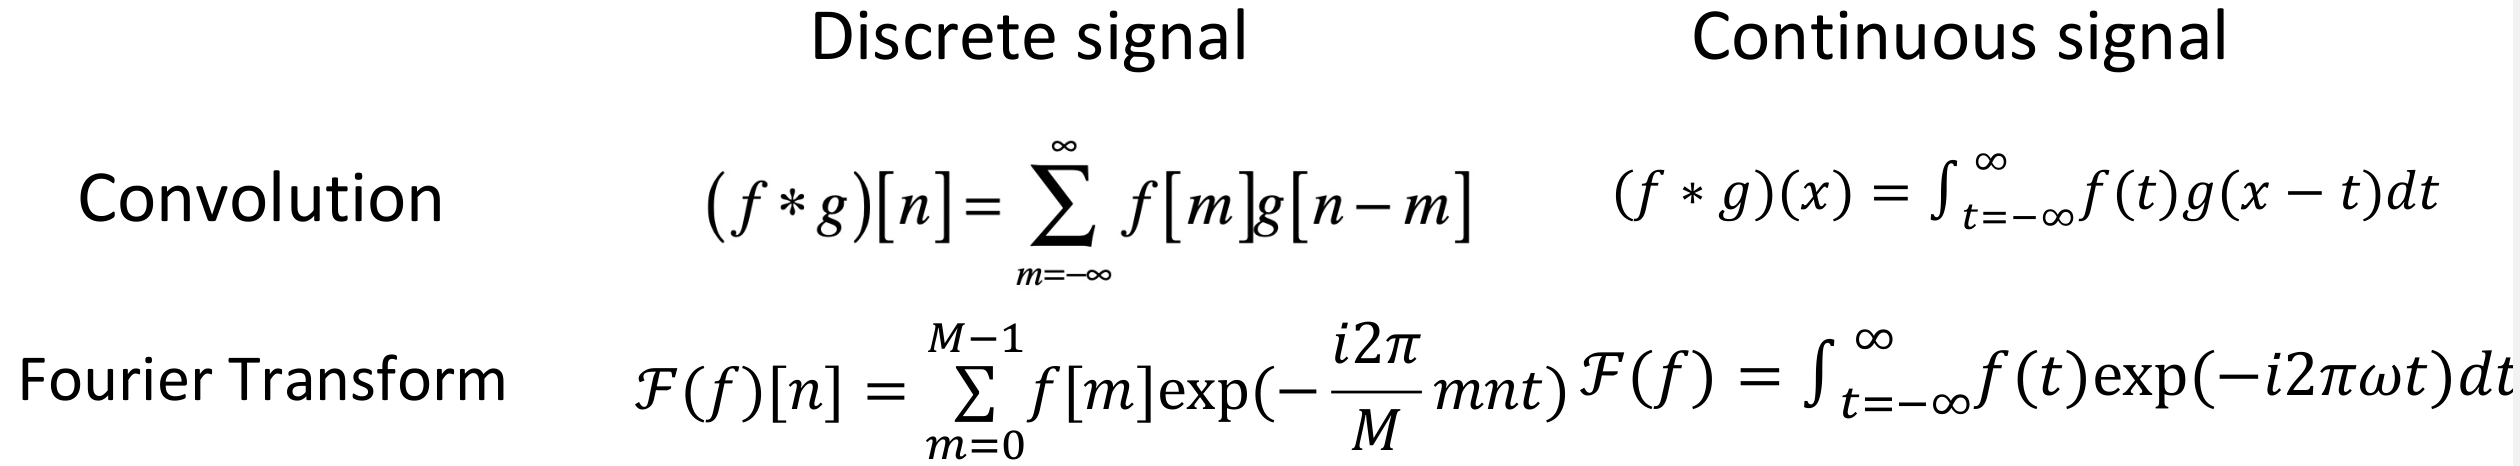
\includegraphics[scale=0.18]{figures/FourierTransform.png}
    \caption{Fourier transform visualization.}
\end{figure}

\clearpage

\subsection{2D Discrete Filter}
\begin{itemize}
    \item Example: 2D moving average over a $ 3 \times 3 $ window:
    $$
    h[i,j] = \frac{1}{9} \sum_{k=-1}^{1} \sum_{l=-1}^{1} f[i+k, j+l]
    $$
\end{itemize}

% --- Placeholders for images "g.png" and "g2.png" ---
\begin{figure}[htbp]
    \centering
    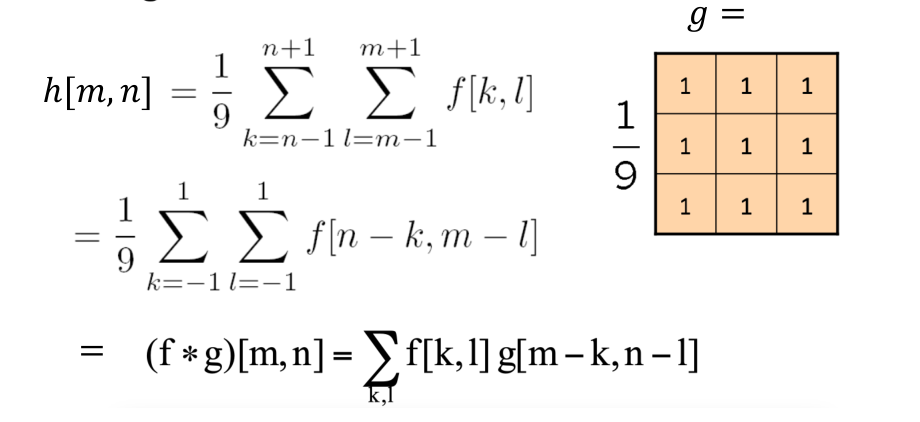
\includegraphics[scale=0.25]{figures/g.png}
    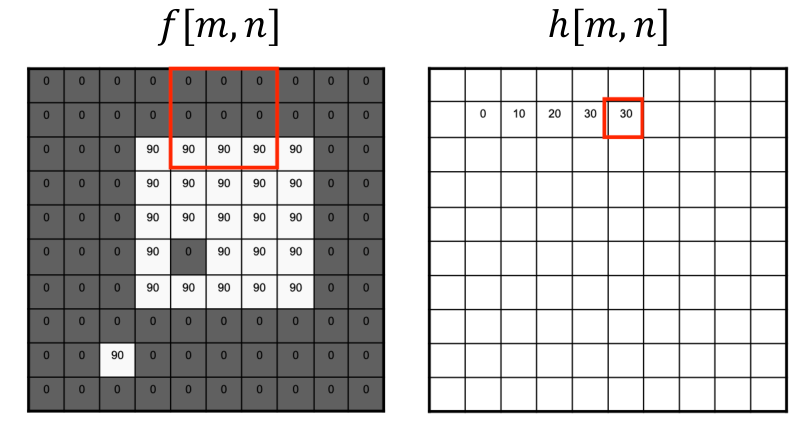
\includegraphics[scale=0.25]{figures/g2.png}
    \caption{Filtering examples.}
\end{figure}

\subsection{Non-linear Filtering}
\begin{itemize}
    \item Example: \textbf{Binarization via Thresholding}:
    $$
    h(x,y) = 
    \begin{cases} 
    255 & \text{if } f(x,y) > T \\
    0   & \text{otherwise}
    \end{cases}
    $$
\end{itemize}

% --- Placeholder for image "BinarizationviaThresholding.png" ---
\begin{figure}[htbp]
    \centering
    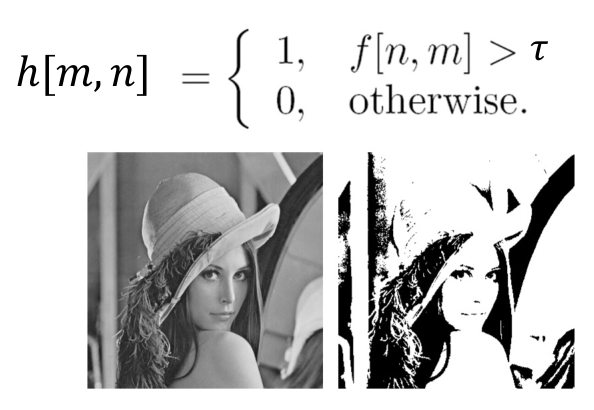
\includegraphics[scale=0.4]{figures/BinarizationviaThresholding.png}
    \caption{Binarization example.}
\end{figure}